\documentclass[ngerman]{beamer}

\usepackage{lmodern}
\usepackage[utf8]{inputenc}
\usepackage[T1]{fontenc}
\usepackage[ngerman]{babel}
\usepackage{graphicx}
\usepackage{xcolor}
\usepackage{amsmath}
\usepackage{amsthm}
\usepackage{datetime}

\graphicspath{{./img/}}
\definecolor{halfgray}{gray}{0.55} % chapter numbers will be semi transparent .5 .55 .6 .0


\DeclareMathAlphabet\mathbfcal{OMS}{cmsy}{b}{n}

%% Listings
\usepackage{listings}
\usepackage{sourcecodepro} % now the default typewriter font

\lstset
  { basicstyle=\tiny\ttfamily\footnotesize
  , breaklines=true
  , captionpos=t
  , showstringspaces=false
  , rulecolor=\color{halfgray}
  , commentstyle=\scriptsize
  , numbers=left
  , frameshape={nnY}{n}{n}{Ynn}
  , xleftmargin=2.5em
  , framexleftmargin=2em
  , keywordstyle=\color{blue}
  , backgroundcolor=\color{black!3}
  }

\lstnewenvironment{haskell}[1][]{
    \noindent
    \minipage{\linewidth}
    \vspace{0.5\baselineskip}
    \lstset
        { basicstyle=\footnotesize\ttfamily
        , language=Haskell
        , tabsize=2
        , #1
        }
}{\endminipage}

\usetheme{Szeged}
\usecolortheme{dolphin}
% \usetheme{Goettingen}
\usefonttheme{professionalfonts}
\setbeamercovered{transparent}
\setbeamertemplate{footline}[frame number]


\begin{document}
\title[Haskell Engine]{Modern OpenGL Engine in Haskell}
\subtitle[Konzepte]{Funktionale Konzepte und Implementierungen}
\author{Jan-Philip Loos}
\institute[FH Wedel]{Master of Science\\Informatik\\
\includegraphics[width=3cm]{fhw}}
\date{\protect\formatdate{02}{06}{2015}}
\maketitle
\logo{
\includegraphics[width=0.5cm]{fhw-logo}}

% \frame{\tableofcontents[currentsection]}
\frame{\tableofcontents}
\section{Formale Basis des Rendersystems}
\stepcounter{subsection}
\frame{\sectionpage}

%% MEALY
\begin{frame}
  \frametitle{Mealy Automat}
  \begin{Definition}
    \begin{align}
    \mathbfcal{M} = \left( Q, \Sigma, \Omega, \delta, \lambda, q_0 \right)
    \label{def:mealy-formal}
    \end{align}
    \begin{align*}
    	\text{mit}\\
    	Q &: \text{Endliche Menge von Zuständen} \\\pause
    	\Sigma  &:\text{Endliches Eingabealphabet} \\\pause
    	\Omega  &:\text{Endliches Ausgabealphabet} \\\pause
    	\delta  &:\text{Zustandsübergangsfunktion}\ Q \times \Sigma \rightarrow Q \\\pause
    	\lambda &:\text{Ausgabefunktion}\ Q \times \Sigma \rightarrow \Omega \\\pause
    	q_0 &: \text{Startzustand}
    \end{align*}
  \end{Definition}
\end{frame}

\begin{frame}[fragile]
  \frametitle{Definition in Haskell}
  \begin{block}{Definition Mealy}
    \begin{align*}
    \mathbfcal{M} = \left( Q, \Sigma, \Omega, \delta, \lambda, q_0 \right)
    \label{def:mealy-formal}
  \end{align*}
  \end{block}
  \begin{haskell}[label={lst:haskell-mealy},caption={[Definition Mealy in Haskell]Definition Mealy in Haskell\protect\footnotemark}]
newtype Mealy a b = Mealy {
  runMealy :: a -> (b, Mealy a b)
}
  \end{haskell}
  \footnotetext{https://hackage.haskell.org/package/machines/}
\end{frame}

\begin{frame}[fragile]
  \frametitle{Monadische Erweiterung von {\ttfamily Mealy}}
  \begin{haskell}[label={lst:haskell-mealy},caption={[Monadische Mealy]Monadische Mealy}]
newtype MealyT m a b = MealyT {
  runMealyT :: a -> m (b, MealyT m a b)
}
  \end{haskell}
\end{frame}

\begin{frame}[fragile]
  \frametitle{Beispielimplementierung eines {\ttfamily MealyT}}

  \begin{haskell}[label={lst:haskell-mealy}]
newtype MealyT m a b = MealyT {
  runMealyT :: a -> m (b, MealyT m a b)
}
  \end{haskell}

  \begin{haskell}
sumAndPrintInput :: Int -> MealyT IO Int Int
sumAndPrintInput q0 = @\pause@ MealyT (\i -> do
  print i
  let sumVal = q0 + i
  return (sumVal,sumAndPrintInput sumVal))
  \end{haskell}
\end{frame}

\begin{frame}[fragile]
  \frametitle{Ausführung von {\ttfamily sumAndPrintInput}}

  \begin{haskell}
sumAndPrintInput :: Int -> MealyT IO Int Int
sumAndPrintInput q0 = MealyT (\i -> do
  print i
  let sumVal = q0 + i
  return (sumVal,sumAndPrintInput sumVal))
  \end{haskell}
  \begin{semiverbatim}
\(\lambda\)> (out0, q1) <- runMealyT (sumAndPrintInput 0) 1\pause
1\pause
\(\lambda\)> print out0 \pause
1\pause
\(\lambda\)> (out1, q2) <- runMealyT q1 42\pause
42\pause
\(\lambda\)> print out1\pause
43
  \end{semiverbatim}
\end{frame}

\begin{frame}

  \frametitle{Kategorien für {\ttfamily MealyT}}

  \begin{itemize}
    \item {\ttfamily Functor}
    \item {\ttfamily Applicative}
    \item {\ttfamily Profunctor}
    \item {\ttfamily Category}
    \item {\ttfamily Semigroup}
    \item {\ttfamily Arrow}
    \item {\ttfamily ArrowChoice}
  \end{itemize}
\end{frame}

\begin{frame}[fragile]
  \frametitle{{\ttfamily Functor} Instanz für {\ttfamily MealyT}}

  \begin{haskell}
instance Monad m => Functor (MealyT m a) where
  fmap :: (b -> c) -> MealyT m a b -> MealyT m a c
  @\pause@fmap f (MealyT run) = MealyT (run >=> \(o,sys') ->
    return (f o, fmap f sys'))
  \end{haskell}\pause

  \begin{haskell}[mathescape, caption={[Anwndung Functor]Anwendung Functor}]
$\lambda$> :t fmap odd (sumAndPrintInput 0)
fmap odd (sumAndPrintInput 0) :: MealyT IO Int Bool
  \end{haskell}

\end{frame}

\begin{frame}
  \frametitle{\ttfamily RenderSystem}
  \begin{block}{\ttfamily RenderSystem}
    {\ttfamily RenderSystem} = {\ttfamily MealyT}
  \end{block}
\end{frame}

\section{Anwendung}
\stepcounter{subsection}
\frame{\sectionpage}
\begin{frame}
  \frametitle{Physically Based Rendering}
  \begin{itemize}
    \item<1-> {physikalisches Oberflächenmaterial- \\und Beleuchtungskonzept}
    \item<2-> {allgemeingültige und nachvollziehbare Parameter}
    \item<3-> {kein festes Formelwerk}
    \item<4-> {viele mögliche Implementierungen}
    \item<5-> {Paradigma}
  \end{itemize}
\end{frame}

\begin{frame}
  \frametitle{Cook Torrance Modell}
  \begin{itemize}
    \item<1-> {effizientes Reflexionsmodell ($BRDF$)}
    \item<2-> {berücksichtig den Fresnel Effekt}
    \item<3-> {simuliert Mikrofacetten}
  \end{itemize}
  \pause
  \begin{Definition}
    \begin{align}
    	% \caption{Cook-Torrance Illumination}
    	f(\vV,\vL) = \frac{\mathcal{F}(\vV,\vL)D(\vV,\vL)G(\vV,\vL)}{4(\vN \cdot \vV)(\vN \cdot \vL)}
    \end{align}
  \end{Definition}
\end{frame}

\begin{frame}
  \frametitle{Cook Torrance Modell (2)}
  \begin{Definition}

    \begin{align*}
    	f(\vV,\vL) = \frac{\mathcal{F}(\vV,\vL)D(\vV,\vL)G(\vV,\vL)}{4(\vN \cdot \vV)(\vN \cdot \vL)}
    \end{align*}

    \begin{align*}
      \text{mit}\\
      \mathcal{F} &: \text{Fresnel} \\
    	D  &: \text{Mikrofacetten Normalverteilung} \\
    	G  &: \text{Geometrische Abschwächung}
    \end{align*}

  \end{Definition}
\end{frame}

\begin{frame}
  \frametitle{Oberflächenparameter}

  \begin{figure}
    \centering
    \begin{subfigure}{0.24\textwidth}
    	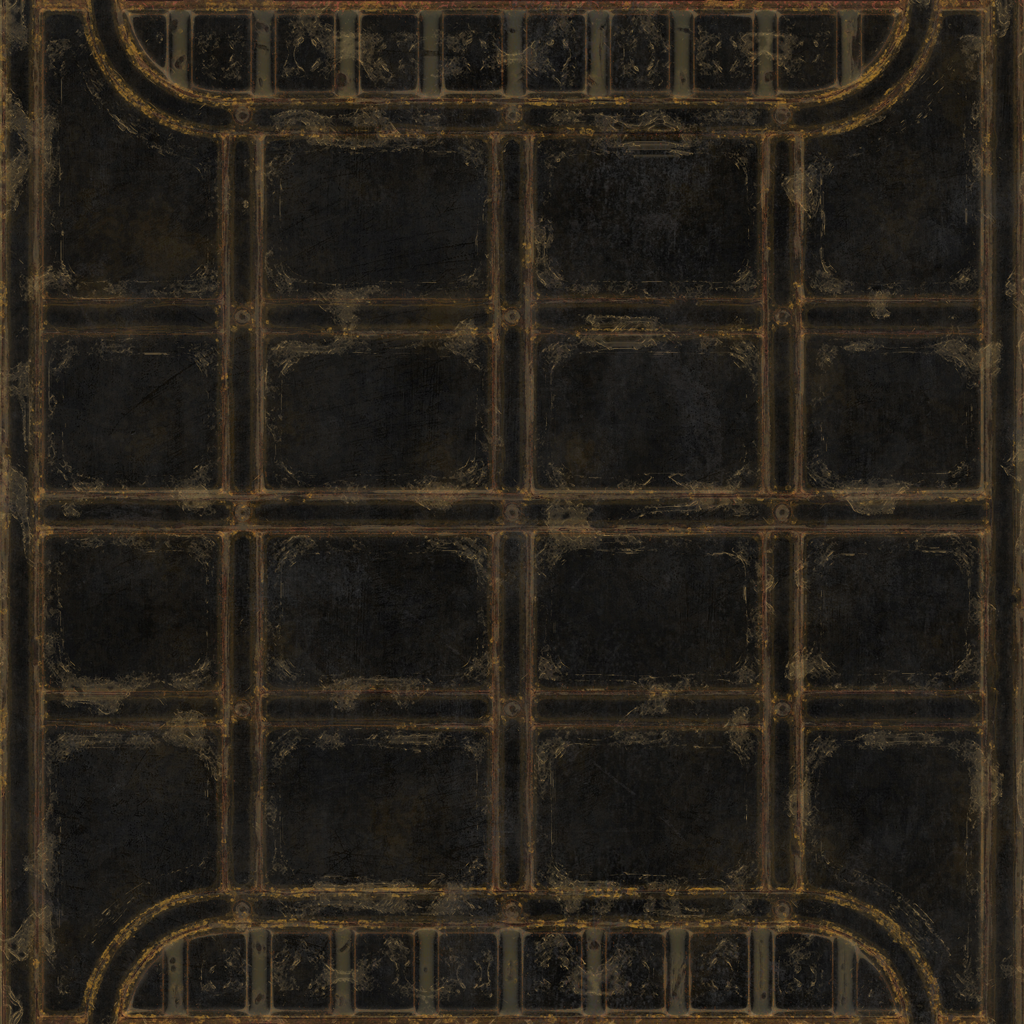
\includegraphics[width=\textwidth]{Door_IronDungeonDoor_1k_alb}
    	\caption{Albedo-Textur}
    \end{subfigure}
    \begin{subfigure}{0.24\textwidth}
    	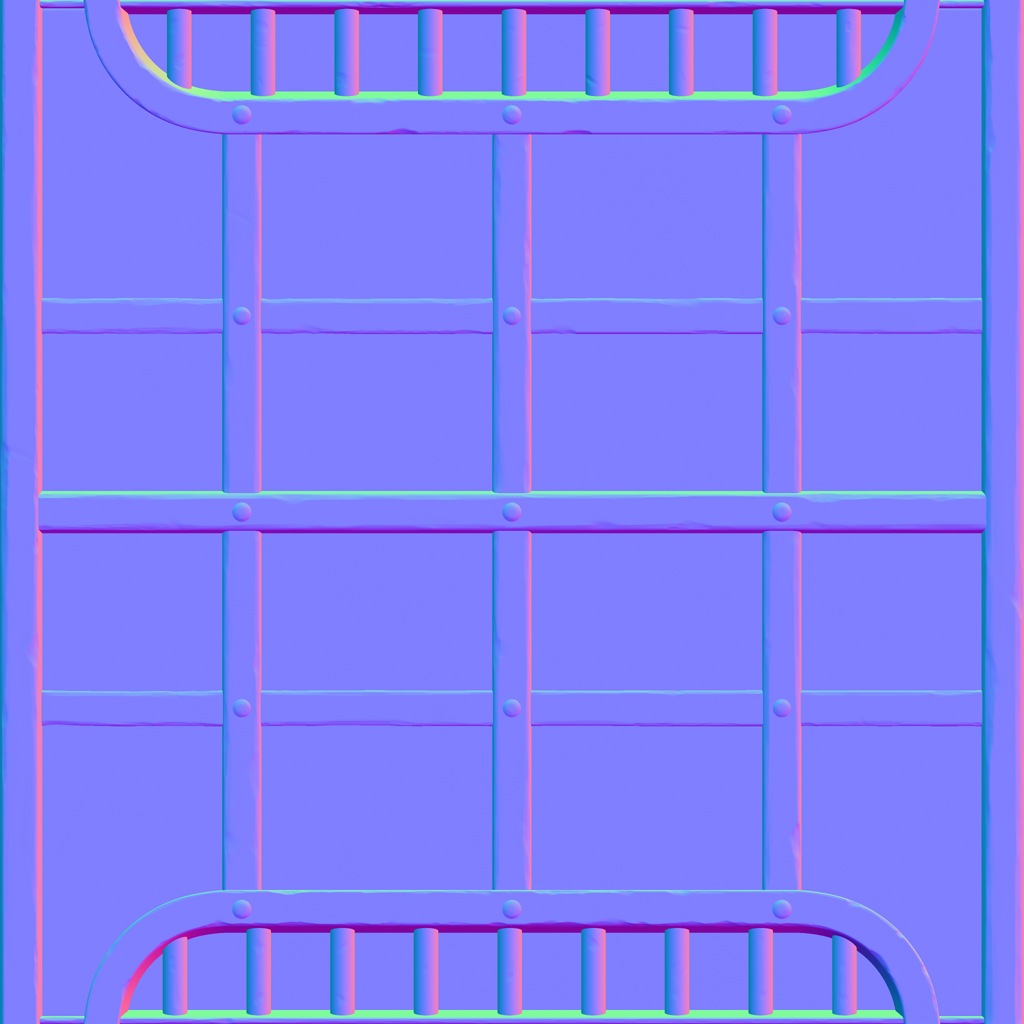
\includegraphics[width=\textwidth]{Door_IronDungeonDoor_1k_n}
    	\caption{Normalen-Textur}
    \end{subfigure}
    \begin{subfigure}{0.24\textwidth}
    	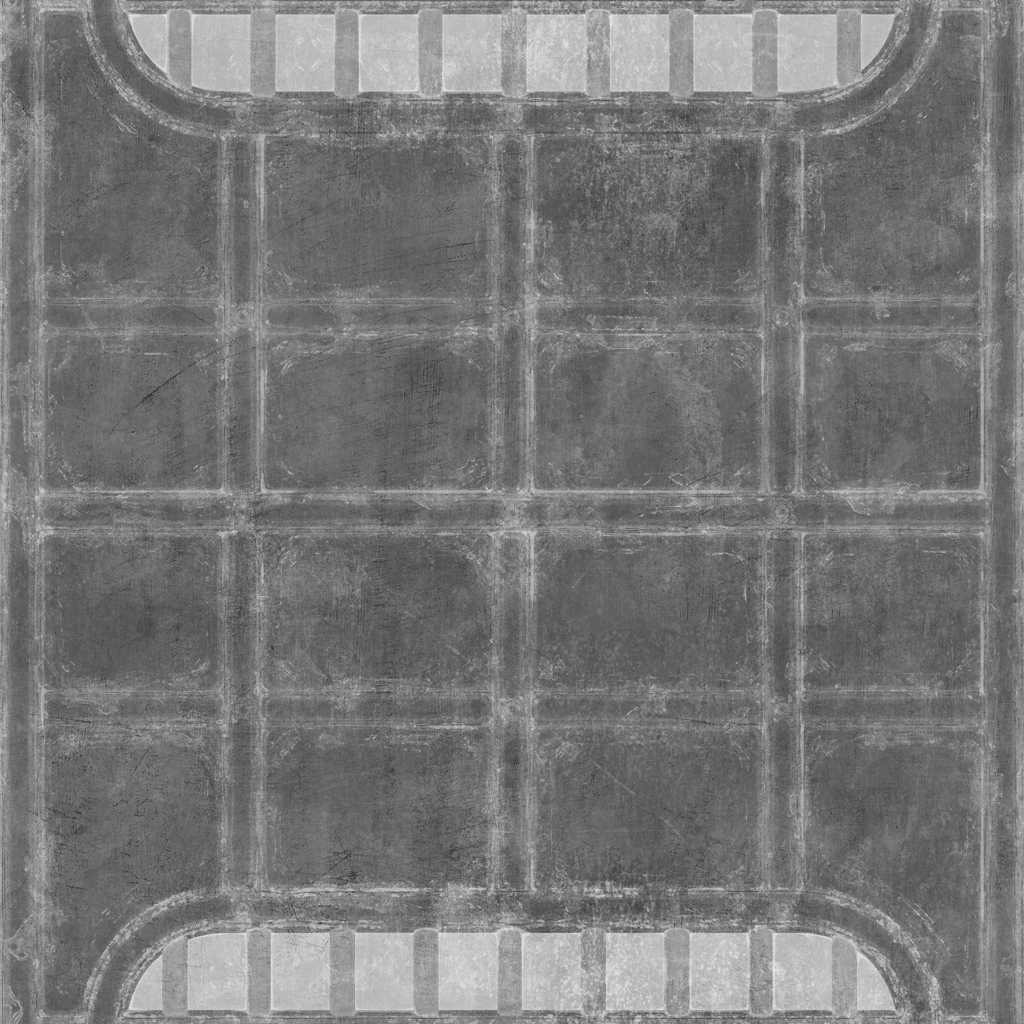
\includegraphics[width=\textwidth]{Door_IronDungeonDoor_1k_rr}
    	\caption{Roughness-Textur}
    \end{subfigure}
    \begin{subfigure}{0.24\textwidth}
    	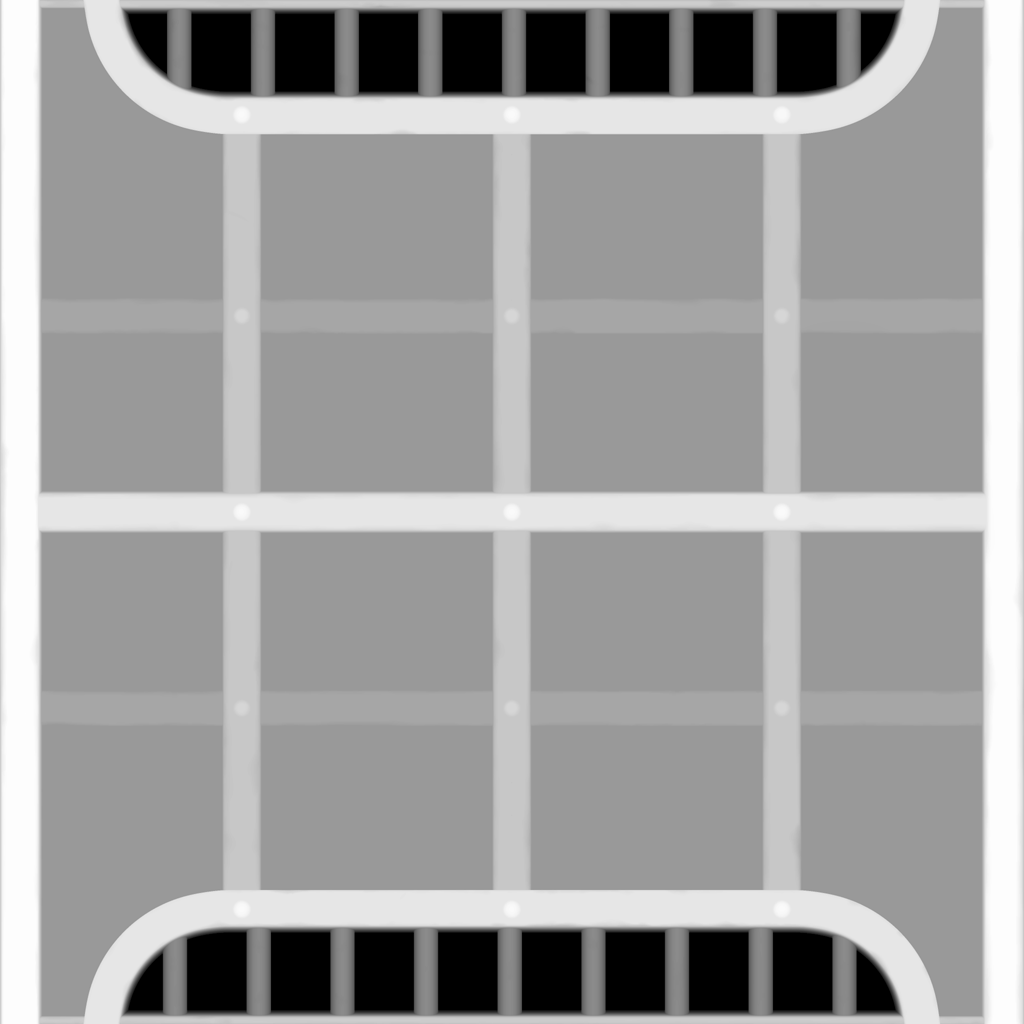
\includegraphics[width=\textwidth]{Door_IronDungeonDoor_1k_h}
    	\caption{Metal-Mask-Textur}
    \end{subfigure}
    \caption{Beispiel eines Textur-Sets}
  \end{figure}

\end{frame}


\section{Demonstration}
\stepcounter{subsection}
\begin{frame}
  \sectionpage
  \centering
  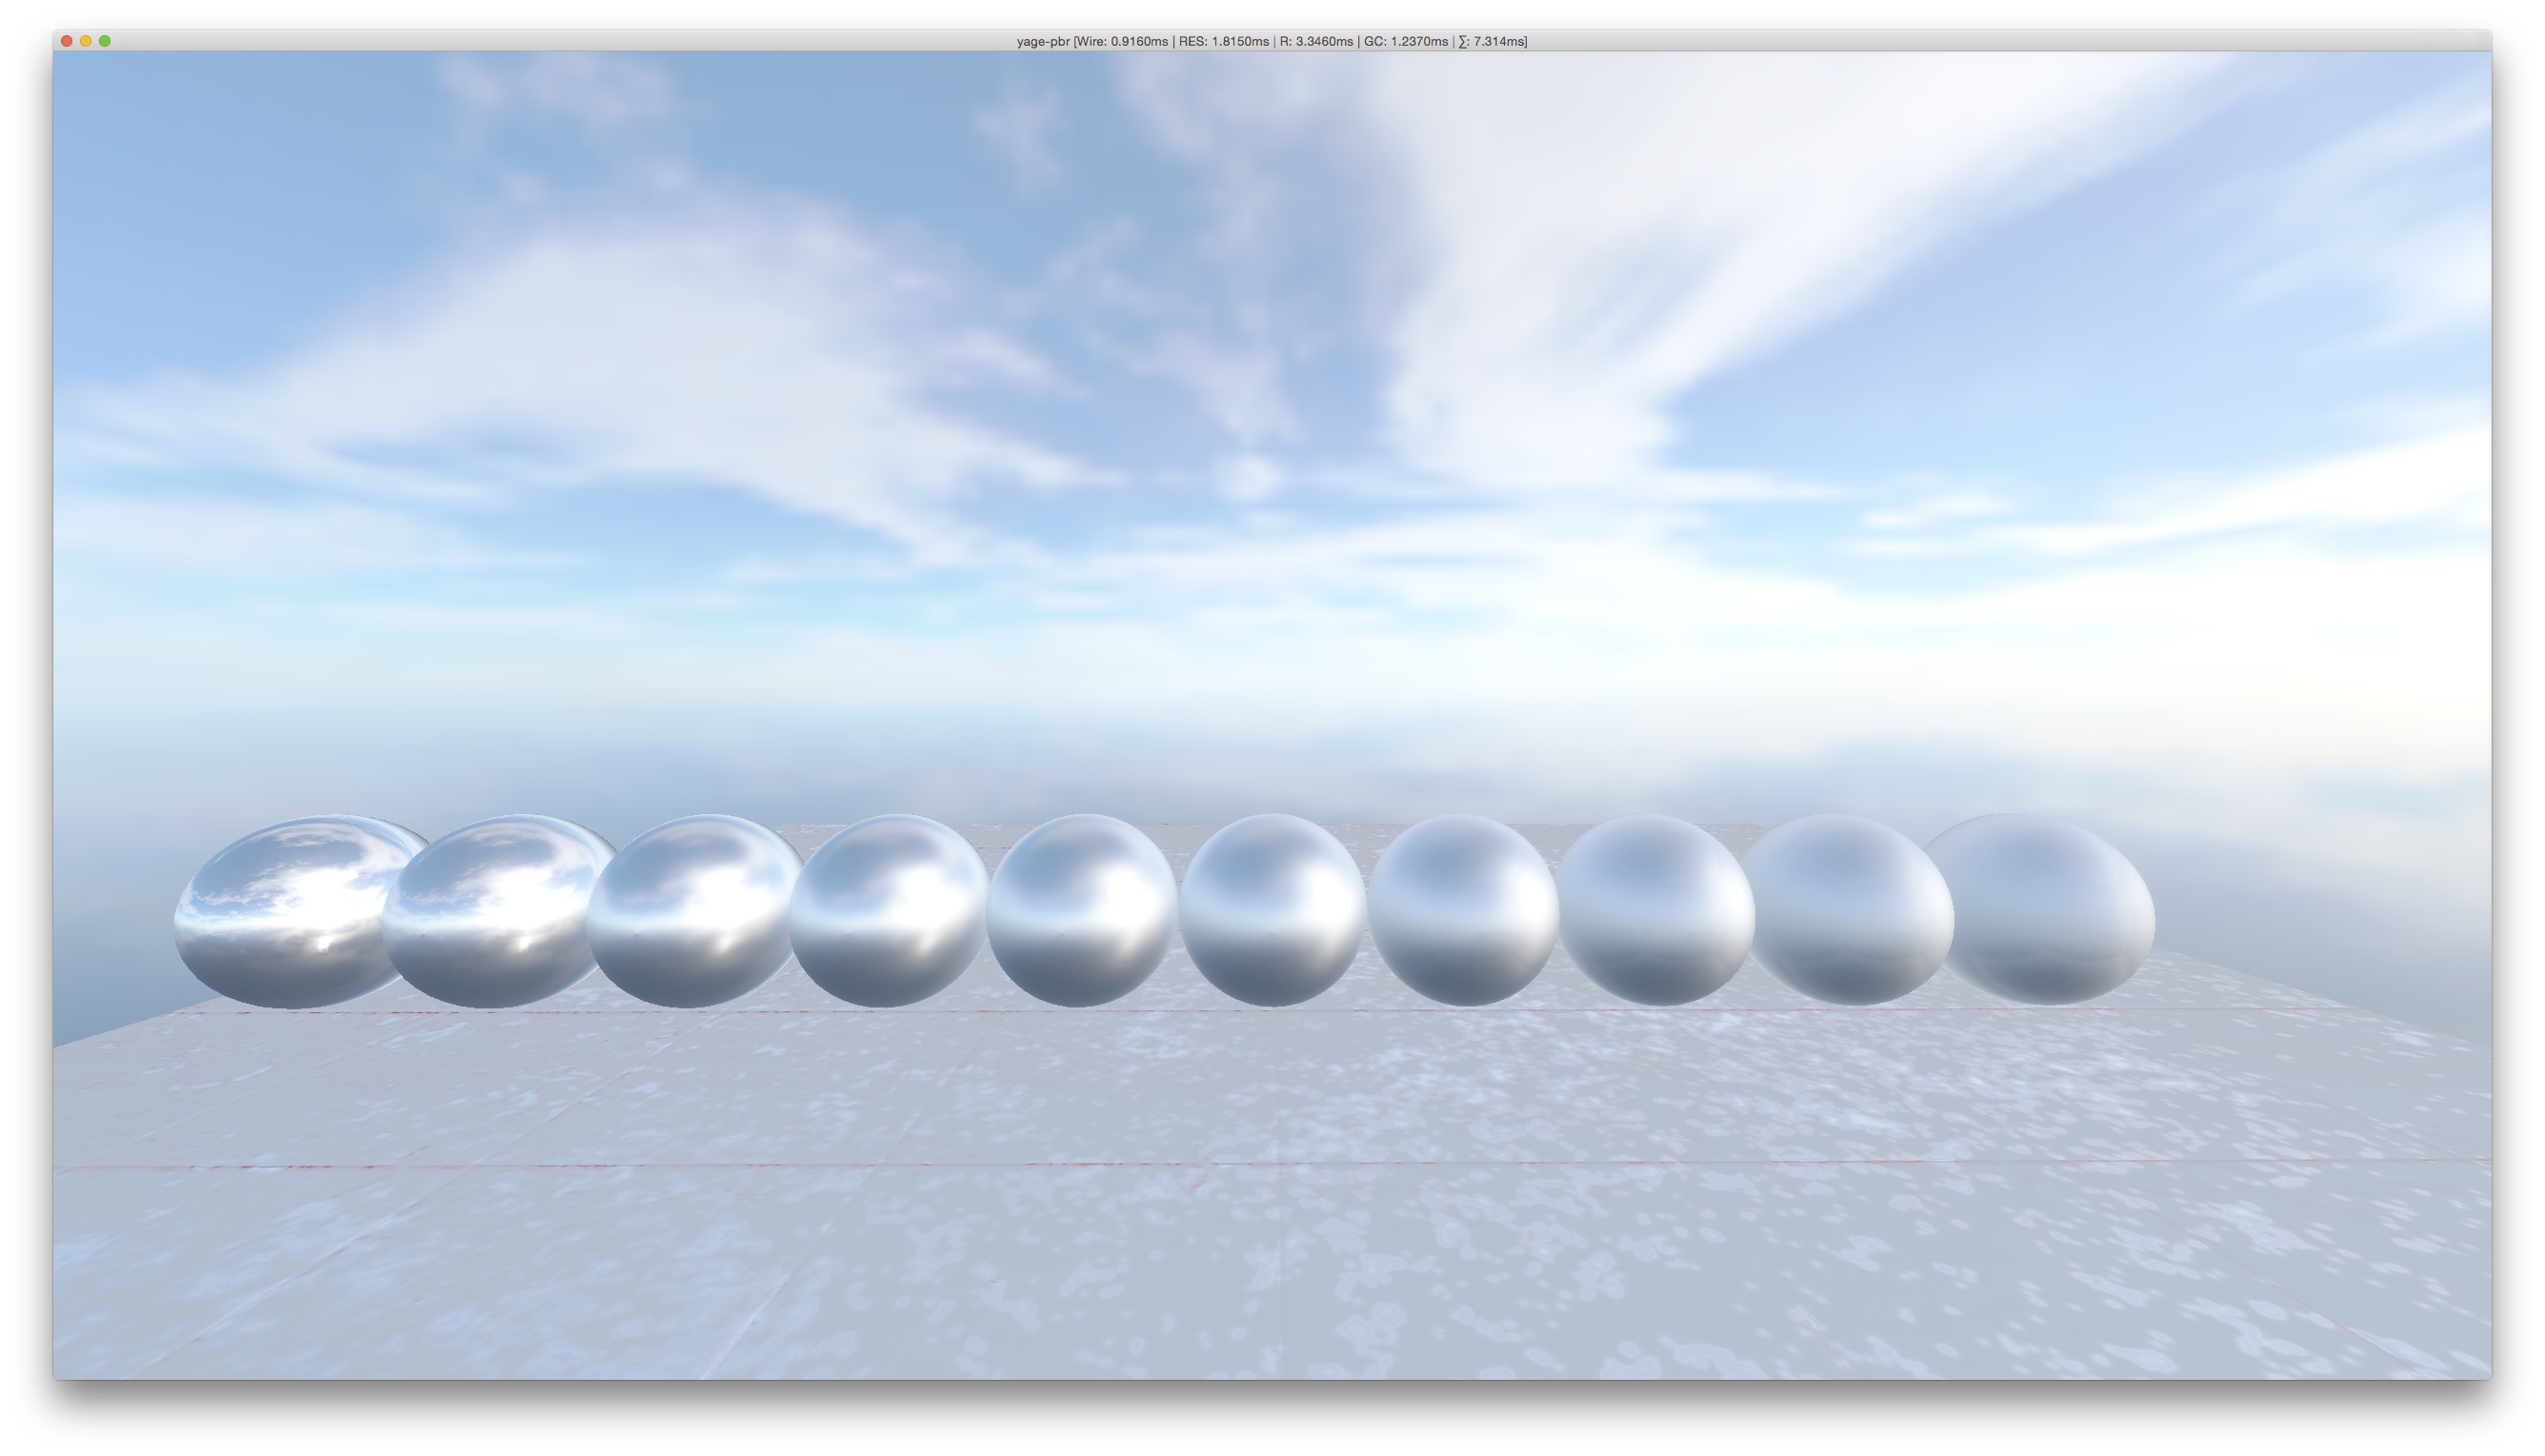
\includegraphics[width=0.8\textwidth]{shots/pbr01}
\end{frame}
\end{document}
